\section{Prototype Implementation for Service Composition}
\label{sec:implementation}

\subsection{System Architecture}
We develop a prototype for our service composition approach to study its performance in the real environments. The system architecture is shown in Figure \ref{fig:lasecalg-implementation-architecture}.

\begin{figure}
\centering
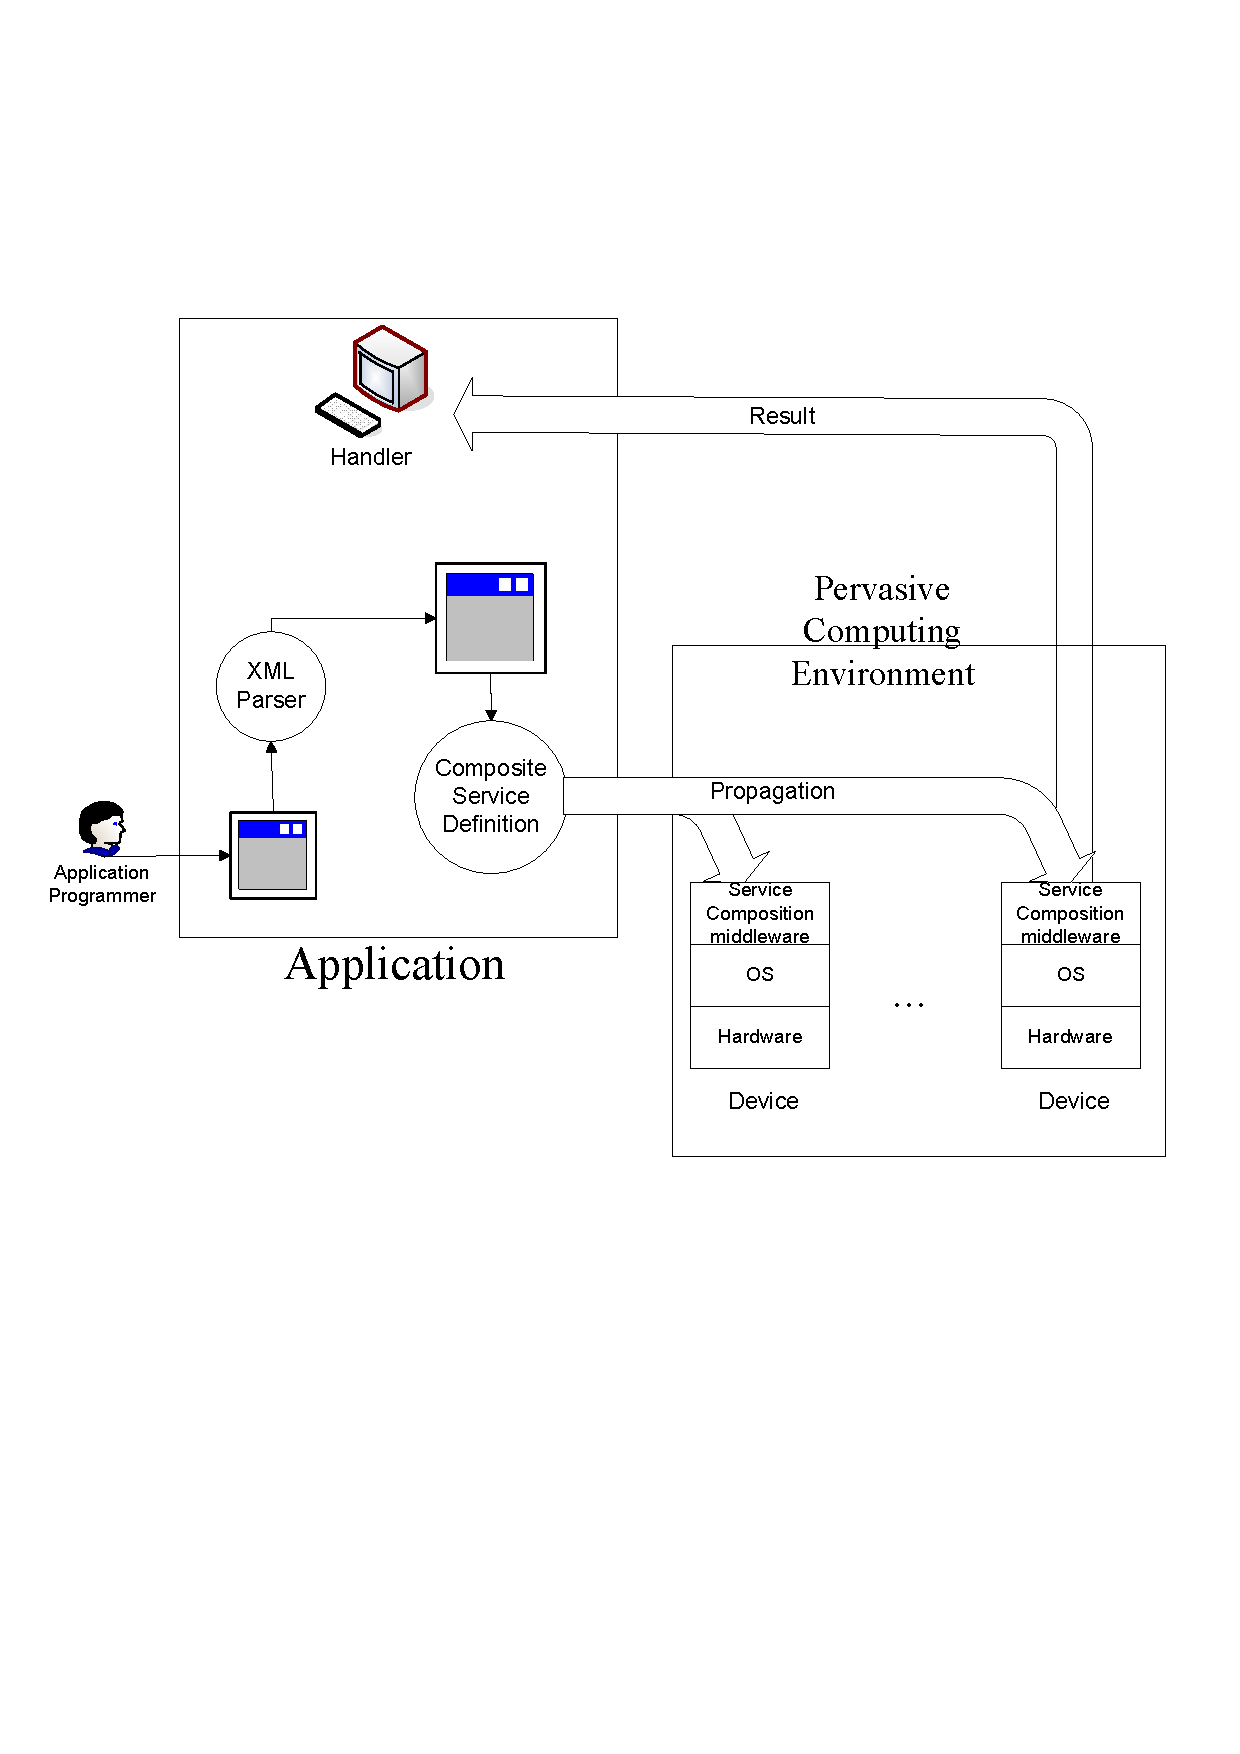
\includegraphics[width=.4\textwidth]{lasecalg-implementation-architecture}
\caption{LASECalg implementation architecture}
\label{fig:lasecalg-implementation-architecture}
\end{figure}

To use our system, users first define service compositions with an XML. In the XML schema, each tag name represents a unique type of service. Each tag may have an optional attribute, namely nodes, which specifies a list of node IDs which provides the corresponding service. If a tag has text, then it represents an argument to be passed to a service. Service composition hierarchy is defined by the hierarchical structure in the XML tags.

\begin{lstlisting}[caption=A simple service for switching on TV, label=lst:watchTV]
<WatchTV>
	<TVOn>
		<TVSwitch nodes="23, 36">
			<operation>on</operation>
		</TVSwitch>
	</TVOn>
	<LightDim>
		<LightSwitch nodes="22, 35">
			<intensity>5</intensity>
		</LightSwitch>
	</LightDim>
</WatchTV>
\end{lstlisting}

A simple example of a service for watching TV is shown in Listing \ref{lst:watchTV}. In this example, the 'WatchTV' service is composed of two high level sub-services: 'TVOn' and 'LightDim'. Each of the service can in turn, be provided by the corresponding TV switch and light switch services with the proper arguments. By using our XML schema, we can easily deploy and test different types of application scenarios in our testbed simply by re-defining the services and the corresponding nodes which provide such services.

The XML containing the user's defined services will then be parsed and packetized for dissemination into the pervasive computing environment. As shown in Figure \ref{fig:lasecalg-implementation-architecture}, on the pervasive device side, after the devices receive the service specification they will start executing the service composition algorithm and notify the user when the composition process is complete. We use MicaZ / MIB600 as our hardware platform for the sensor nodes. Figure \ref{fig:lasecalg-implementation-hardware} shows our test bed platform.

\begin{figure}
\centering
\subfloat[Sensor nodes]{
	\subfloat{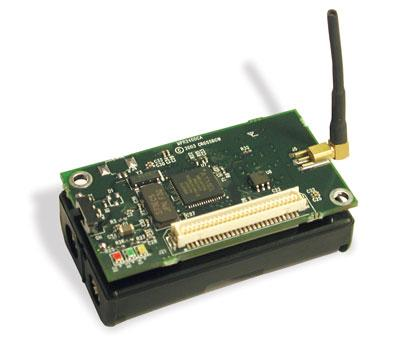
\includegraphics[width=.2\textwidth]{micaz.jpg}}
	\subfloat{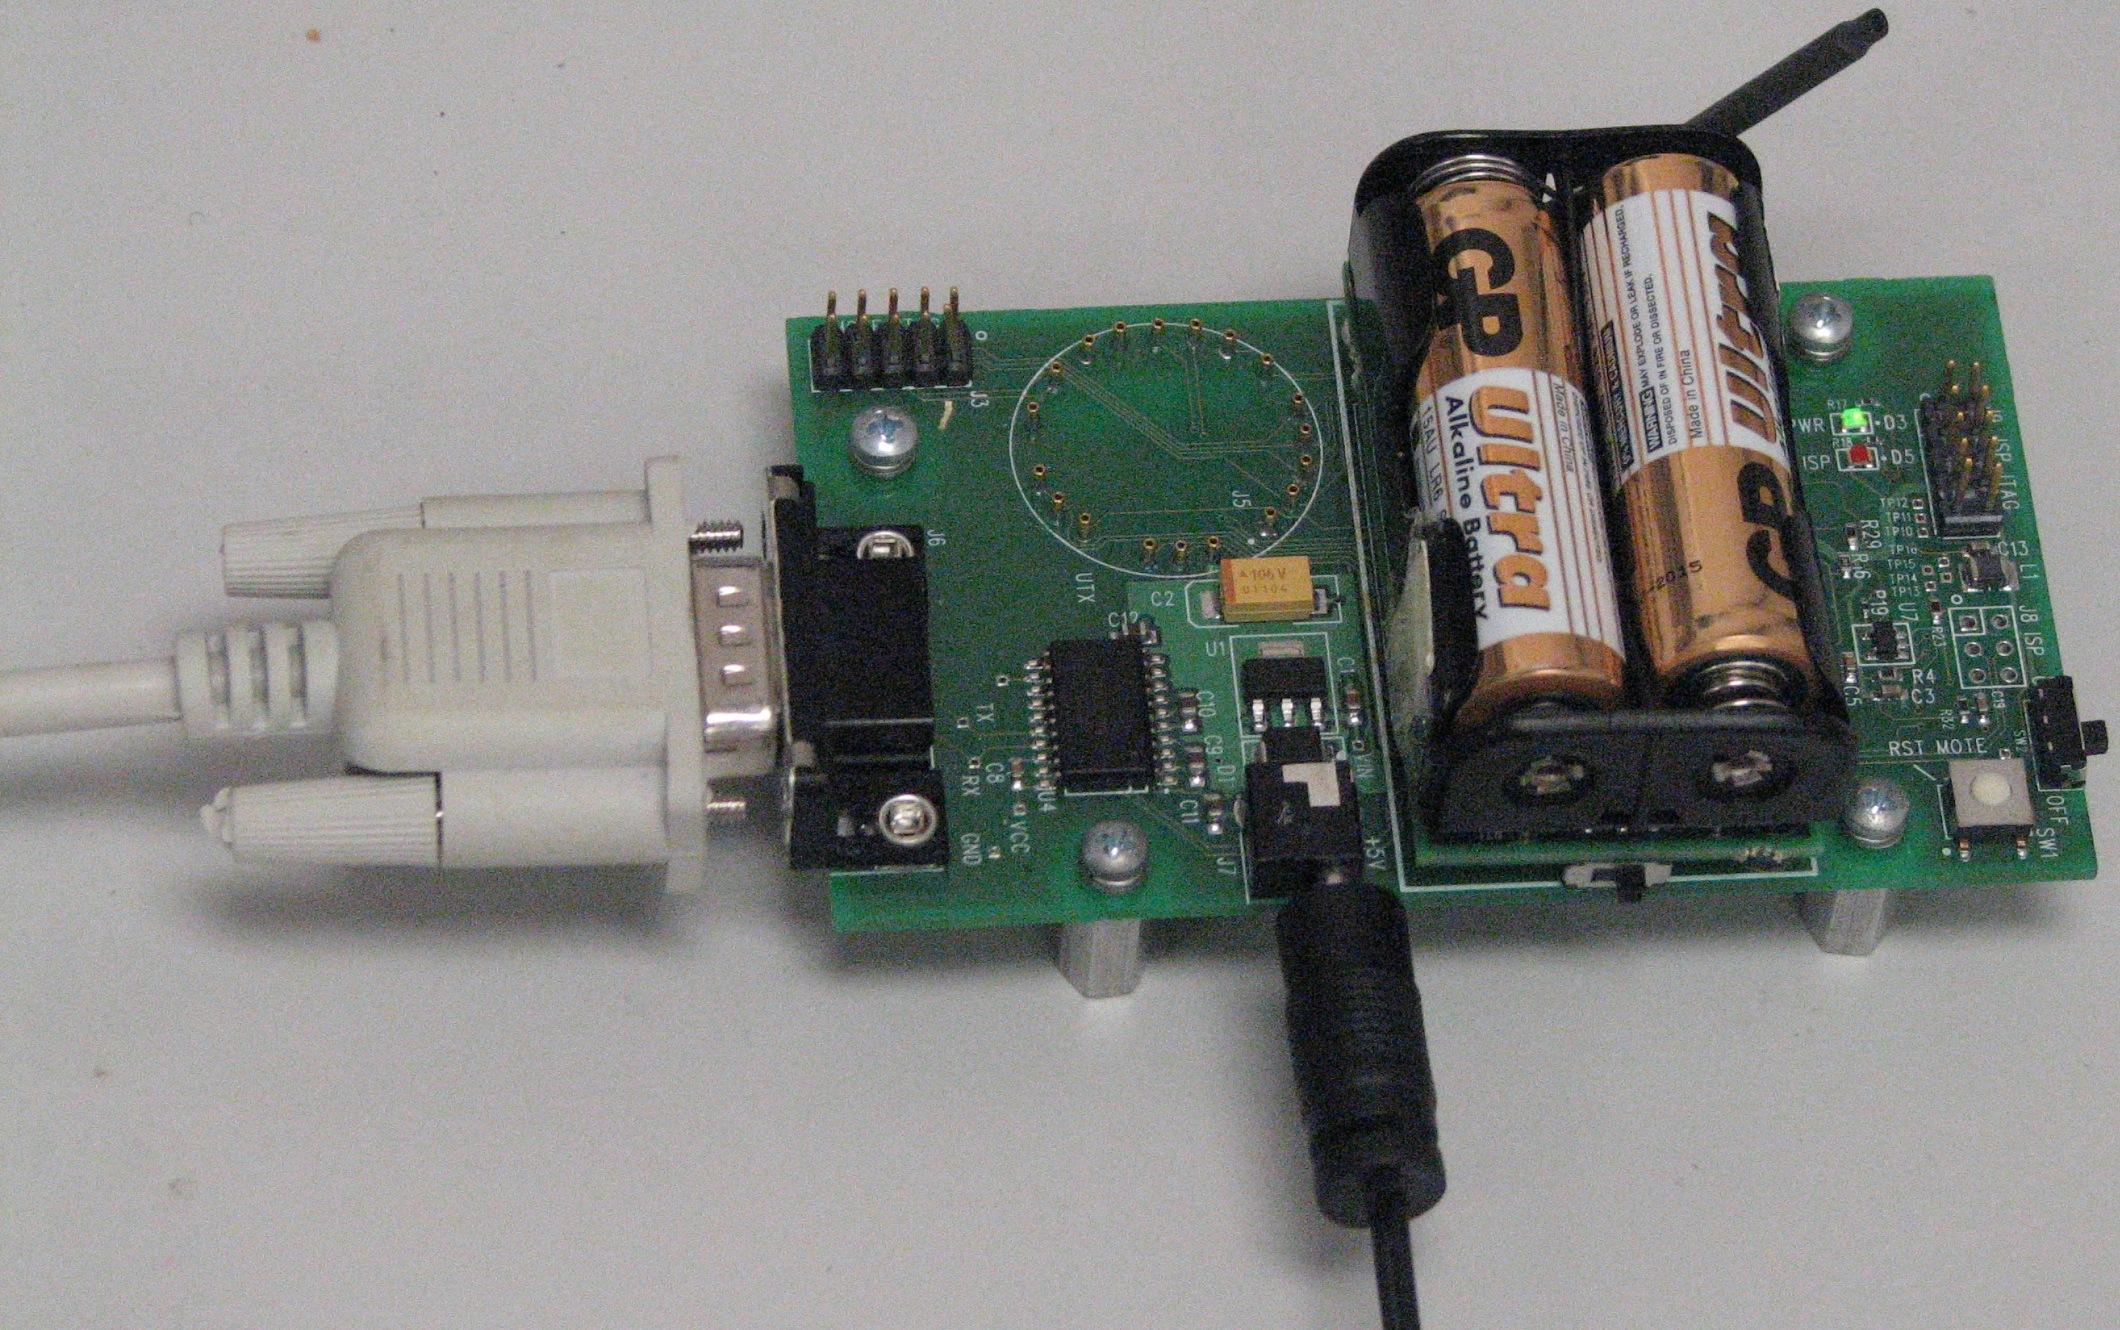
\includegraphics[width=.2\textwidth]{mib510.jpg}}}
\qquad
\subfloat[Test bed setup]{\label{fig:deploy-testbed}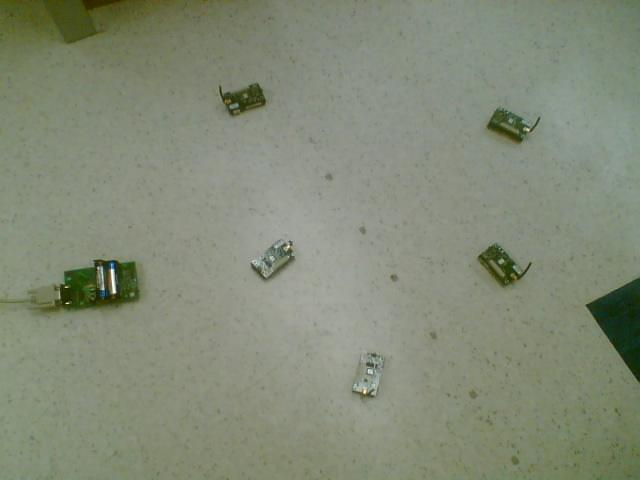
\includegraphics[width=.4\textwidth]{testbed.jpg}}
\caption{Test bed platform}
\label{fig:lasecalg-implementation-hardware}
\end{figure}

\subsection{Experiments}
We conducted experiments based on our prototype.  We pre-defined a number of services in our XML for each sensor node in our testbed. Similar to our simulation, we use CEN as a reference for performance comparison. We implemented CEN based on existing CTP in TinyOS where the nodes will send their available services to sink for composition. We use message cost and delay as metrics for the experiments and study the performance according to \(|V_r |\)of SCP. The experimental results for message cost are shown in the Figures \ref{fig:lasecalg-experiments-cost}. The data in Sub-figure \ref{fig:lasecalg-exp-cost10-2k} are obtained from experiments on 10 pre-defined services while the data in Sub-figure \ref{fig:lasecalg-exp-cost20-2k} are obtained from experiments on 20 pre-defined services. In addition, we tested the two cases for LASECalg where the number of hops, k, is equal to 2 and 4, as indicated in the figures. Compared to CEN, LaSeC can reduce the message cost by over 50\%. This is primarily because of LaSeC's decentralized service composition. Unlike CTP where all the messages must be transmitted to the sink, a lot of messages in LaSeC are processed in-network. In addition, LaSeC also scale better when the number of services increases. This is because when the number of services increases, the number of messages to be sent to the sink in CEN will increase accordingly. This inevitably causes a lot of packet collisions and message re-transmission.  We believe such cost saving is of particular significance when considering the fact that many devices in pervasive computing environment are battery-powered.

The number of hops, k, has certain effect on the cost. With larger value of k, the message cost of LASECalg is also slightly increased. This is because the nodes will talk to more nodes when trying to compose the services.

\begin{figure}
\centering
\subfloat{\label{fig:lasecalg-exp-cost10-2k}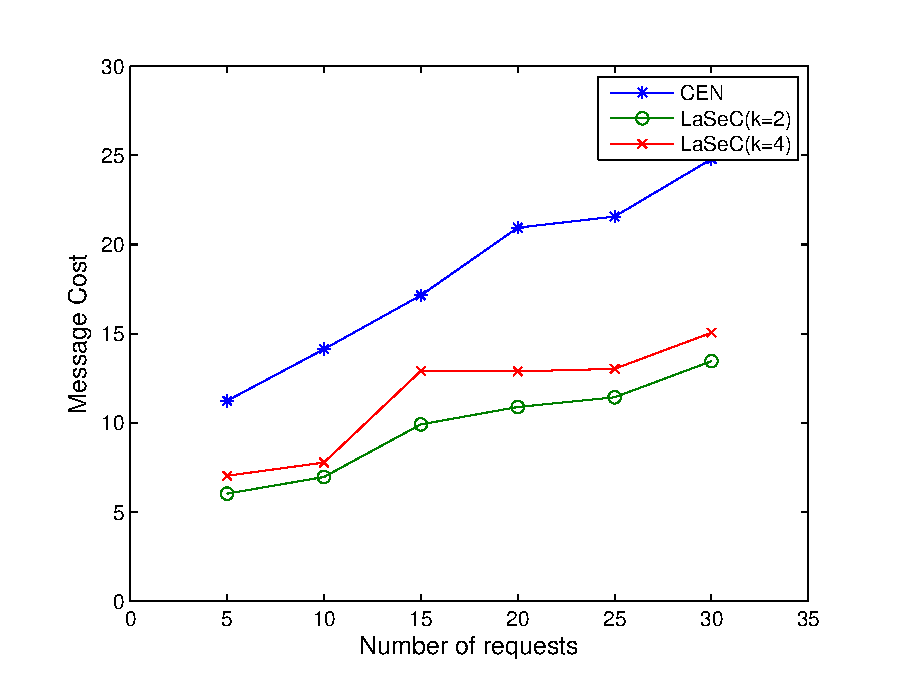
\includegraphics[width=.24\textwidth]{exp-cost10-2k}}
\subfloat{\label{fig:lasecalg-exp-cost20-2k}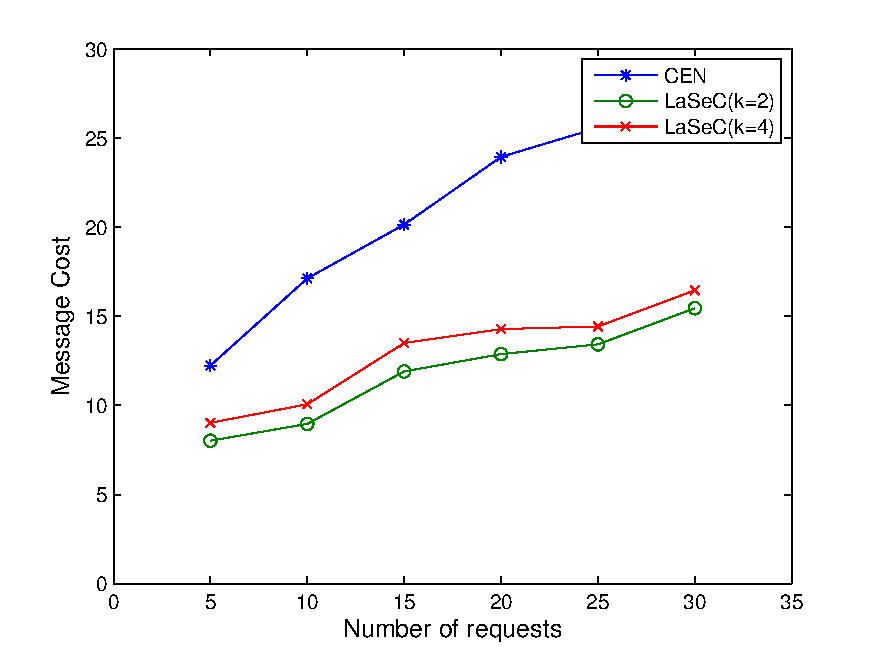
\includegraphics[width=.24\textwidth]{exp-cost20-2k}}
\caption{Message cost}
\label{fig:lasecalg-exp-cost}
\end{figure}

The experimental results for message delay are illustrated in Figure \ref{fig:lasecalg-exp-delay}. Similarly, the data in Sub-figure \ref{fig:lasecalg-exp-delay10-2k} are obtained from experiments on 10 pre-defined services while the data in Sub-figure \ref{fig:lasecalg-exp-delay20-2k} are obtained from experiments on 20 pre-defined services.  We can see that on average, LaSeC achieves smaller delay, especially when there are more services in the environment. This is because in CEN, the delay is primarily introduced by message collision and packet retransmission when the devices try to deliver messages to the sink. On the other hand, the decentralized service composition in LaSeC allows more data to be processed in-network and hence, reduces the chance of packet collision.

The number of hops, k, has small effect on the delay. With larger value of k, the delay is shorter. This is because with more hops, it's easier for the nodes to find necessary service providers for service composition.

\begin{figure}
\centering
\subfloat{\label{fig:lasecalg-exp-delay10-2k}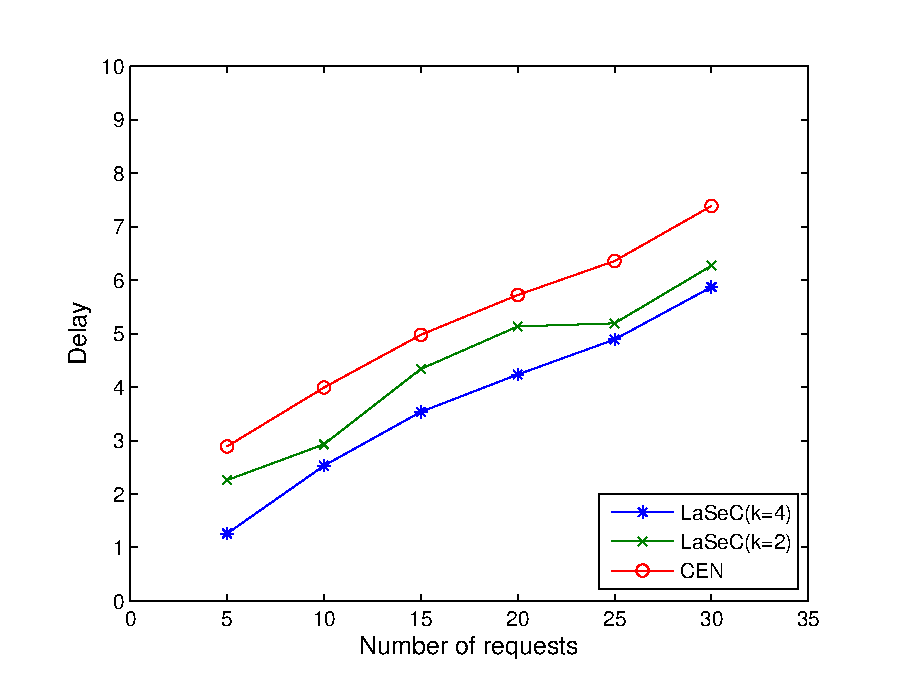
\includegraphics[width=.24\textwidth]{exp-delay10-2k}}
\subfloat{\label{fig:lasecalg-exp-delay20-2k}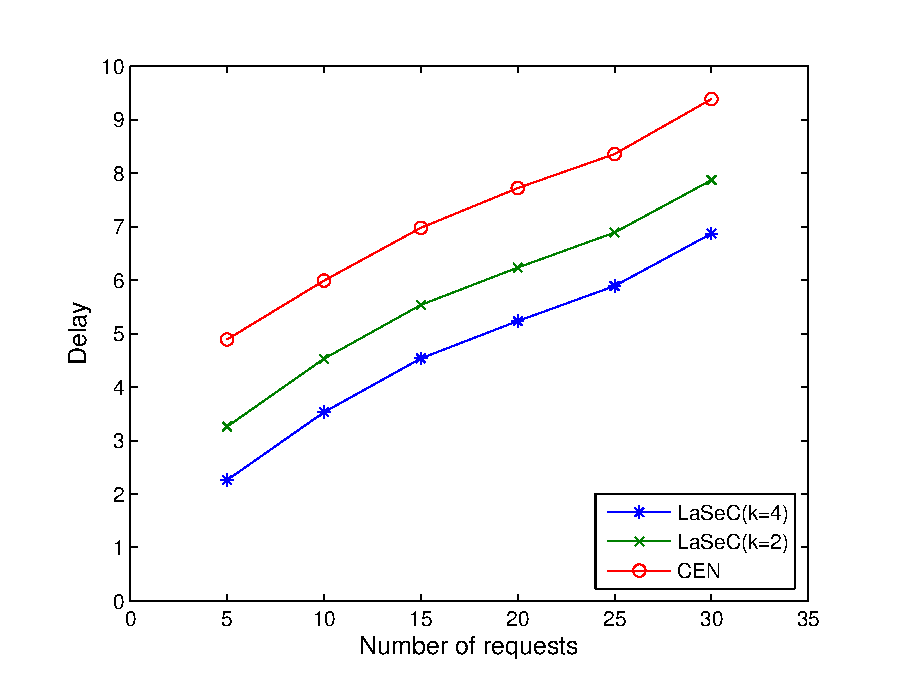
\includegraphics[width=.24\textwidth]{exp-delay20-2k}}
\caption{Message delay}
\label{fig:lasecalg-exp-delay}
\end{figure}